% ============================================================================
%  Problems: รูปสามมิติ (3D Shapes)
%  Ordered from easy (basic) → intermediate.
%  Shared by exercise.tex and answer-key.tex
% ============================================================================

% --- Part 1: พื้นฐาน (Basic) ---
\examsection{ตอนที่ 1: พื้นฐาน — ปริมาตรและพื้นที่ผิว}

\problem{
  ลูกบาศก์มีด้านยาว $5$ ซม. จงหาปริมาตรและพื้นที่ผิว
}{
  ปริมาตร $= 5^3 = 125$ ลบ.ซม.

  พื้นที่ผิว $= 6 \times 5^2 = 150$ ตร.ซม.
}

\problem{
  ทรงสี่เหลี่ยมมุมฉากกว้าง $3$ ซม. ยาว $7$ ซม. สูง $4$ ซม.
  จงหาปริมาตรและพื้นที่ผิว
}{
  $V = 3 \times 7 \times 4 = 84$ ลบ.ซม.

  $SA = 2(3\times 7 + 3\times 4 + 7\times 4)
       = 2(21 + 12 + 28) = 2(61) = 122$ ตร.ซม.
}

\problem{
  ปริซึมฐานสามเหลี่ยมมีพื้นที่ฐาน $15$ ตร.ซม. และสูง $10$ ซม.
  จงหาปริมาตร
}{
  $V = A_{\text{base}} \times h = 15 \times 10 = 150$ ลบ.ซม.
}

\problem{
  พีระมิดฐานสี่เหลี่ยมจัตุรัสมีฐานยาวด้านละ $6$ ซม. และสูง $9$ ซม.
  จงหาปริมาตร
}{
  $V = \dfrac{1}{3} \times 6^2 \times 9 = \dfrac{1}{3} \times 36 \times 9 = 108$ ลบ.ซม.
}

% --- Part 2: การประยุกต์ (Intermediate) ---
\examsection{ตอนที่ 2: การประยุกต์ — ทรงกระบอก กรวย ทรงกลม}

\problem{
  ทรงกระบอกมีรัศมีฐาน $7$ ซม. และสูง $10$ ซม.
  จงหาปริมาตร ($\pi \approx \frac{22}{7}$)
}{
  $V = \pi r^2 h = \dfrac{22}{7} \times 49 \times 10 = 1{,}540$ ลบ.ซม.
}

\problem{
  ทรงกระบอกมีรัศมีฐาน $7$ ซม. และสูง $5$ ซม.
  จงหาพื้นที่ผิวทั้งหมด ($\pi \approx \frac{22}{7}$)
}{
  $SA = 2\pi r^2 + 2\pi rh
       = 2 \times \dfrac{22}{7} \times 49 + 2 \times \dfrac{22}{7} \times 7 \times 5$

  $= 308 + 220 = 528$ ตร.ซม.
}

\problem{
  กรวยมีรัศมีฐาน $3$ ซม. และสูง $4$ ซม.
  จงหาปริมาตรและสูงเอียง ($\ell$)
}{
  $V = \dfrac{1}{3}\pi r^2 h = \dfrac{1}{3}\pi (9)(4) = 12\pi$ ลบ.ซม.

  $\ell = \sqrt{r^2 + h^2} = \sqrt{9 + 16} = \sqrt{25} = 5$ ซม.
}

\problem{
  กรวยมีรัศมีฐาน $6$ ซม. และสูงเอียง $10$ ซม.
  จงหาพื้นที่ผิวทั้งหมด
}{
  $SA = \pi r^2 + \pi r \ell = 36\pi + 60\pi = 96\pi$ ตร.ซม.
}

\problem{
  ทรงกลมมีรัศมี $7$ ซม. จงหาปริมาตรและพื้นที่ผิว
  ($\pi \approx \frac{22}{7}$)
}{
  $V = \dfrac{4}{3}\pi r^3 = \dfrac{4}{3} \times \dfrac{22}{7} \times 343
      = \dfrac{30{,}184}{21} \approx 1{,}437.3$ ลบ.ซม.

  $SA = 4\pi r^2 = 4 \times \dfrac{22}{7} \times 49 = 616$ ตร.ซม.
}

\problem{
  ทรงกลมลูกหนึ่งมีพื้นที่ผิว $= 100\pi$ ตร.ซม.
  จงหาปริมาตรของทรงกลมนี้
}{
  $4\pi r^2 = 100\pi \;\Rightarrow\; r^2 = 25 \;\Rightarrow\; r = 5$ ซม.

  $V = \dfrac{4}{3}\pi (125) = \dfrac{500}{3}\pi$ ลบ.ซม.
}

% --- Part 3: ระดับ สอวน. (POSN Level) ---
\examsection{ตอนที่ 3: ระดับข้อสอบ สอวน.}

\problem{
  (ข้อสอบจริงปี 67 ข้อ 18) ให้ทรงกรวยตัน รัศมี 9 เซนติเมตร สูงตรง 12 เซนติเมตร ดังรูป ถ้าตัดกรวยขนานกับแนวราบตามเส้น A 
(จากยอดกรวยแหลมลงมา 4 เซนติเมตร) แล้วหยิบส่วนบนที่มียอดแหลมด้วยนั้นออกไป  
จงหาว่าปริมาตรของกรวยส่วนล่างที่เหลือ มีค่าเป็นกี่เท่าของปริมาตรกรวยเดิม (Hint: ใช้เรื่องสามเหลี่ยมคล้าย)
  \begin{center}
    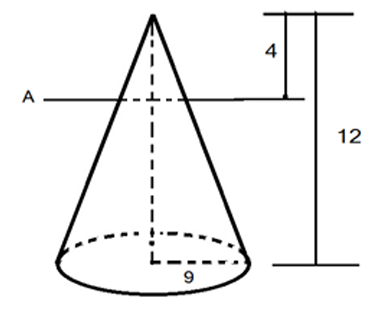
\includegraphics[width=0.35\textwidth]{images/geometry-3d-01.png}
  \end{center}
}{
  $\dfrac{52}{54}$
}